\chapter{Delta potential} \label{chapter-dirac}
In this chapter we will examine the Landau Hamiltonian with a potential perturbation (see definition \ref{defn-perturb-potential}), formally given by the potential $V(x) = \alpha\,\delta_{x_0}$, i.e. the Dirac delta in $x=x_0$ with a coupling constant (\textit{magnitude}) $\alpha \in \R$. Since such a~potential is a~distribution and not a~locally integrable function, the Hamiltonian is rigorously defined as follows.
\begin{defn}[Landau Hamiltonian with a Dirac delta perturbation]
    \label{defn-hamiltonian-dirac}
    \ph{.}\\
    Let $\alpha, b \in \R \setminus \{ 0 \}$ and $x_0 \in \R$. We define a linear operator $H_\alpha$ on $L^2(\R^2)$
    \begin{equation*}
        \big( H_\alpha \psi \big)(x, y) := \left( -\pd{^2}{x^2} + \big( \i\pd{}{y} + bx \big)^2 \right) \; \psi(x,y)
        \quad \text{a.e.\footnotemark on } (\R \setminus \{ x_0 \}) \times \R
    \end{equation*}
    \footnotetext{The pointwise equality is to be understood \textit{almost everywhere} with respect to the Lebesgue measure on $\R^2$.}
    with a domain given by the conditions
    \begin{gather*}
        \psi \in W^{1,2}(\R^2) \; \cap \; W^{2,2}\big( \,(\R \setminus \{ x_0 \}) \times \R \, \big) \: ,
        \\[5pt]
        \lim_{x \to x_0 +} \pd{}{x}\psi(x,y)\; - \lim_{x \to x_0 -} \pd{}{x}\psi(x,y) = \alpha \lim_{x \to x_0} \!\psi(x, y)
        \quad \text{for a.e. } y \: ,\footnotemark
        \\[5pt]
        \int_{\R^2} x^2 \, \big|\, \psi(x,y) \,\big|^2 \, \d{x}\d{y} < \infty \: .
    \end{gather*}
    \footnotetext{The equality holds for \textit{almost every} $y$ and $\lim_{x\to x_0}$ means the \textit{essential} limit with respect to the Lebesgue measure on $\R$.}
\end{defn}
By an approach analogous to \eqref{eqn-vague-direct-integral-decomp}, one can show that $H_\alpha$ is unitarily equivalent to a direct integral:
\begin{equation*}
    H_\alpha \simeq \int^\oplus_\R \Hf_\alpha(p) \d{p} \: ,
\end{equation*}
where $\Hf_\alpha(p)$ is a fibre Hamiltonian satisfying very similar conditions to those of~$H_\alpha$, that is, for almost every $p \in \R$:
\begin{gather*}
    \big( \Hf_\alpha(p) \, \varphi \big)(x)
    = -\varphi''(x)
    + \big( b \, x + p \big)^2 \, \varphi(x) \: ,
    \numberthis\label{eqn-dirac-fibre-hamiltonian}
    \\[15pt]
    \varphi \in W^{1,2}(\R) \; \cap \; W^{2,2}( \R \setminus \{ x_0 \}) \: ,
    \\[5pt]
    \lim_{x \to x_0+} \varphi'(x) - \lim_{x \to x_0-} \varphi'(x) = \alpha \, \lim_{x \to x_0} \varphi(x),
    \\[3pt]
    \int_\R x^2 \, |\varphi(x)|^2 \d{x} < \infty \: .
\end{gather*}
Sometimes, we will want to explicitly specify not only $\alpha$ and $p$, but also the value of $x_0$. In that case, we will denote the fibre Hamiltonian as $\Hf_{\alpha, \, x_0}(p)$.

Before we start investigating the spectrum, we need to show that the problem is well-posed, i.e. that the Hamiltonian $H_\alpha$ is self-adjoint and bounded from below. Then we will show that the spectrum of $\Hf_\alpha(p)$ is discrete for every $p$, and only after that we will investigate the continuity of the spectrum of $H_\alpha$.

\section{Well-posedness} \label{section-dirac-well-posedness}
It is straightforward to check that the fibre Hamiltonian is bounded from below:
\begin{align*}
    (\varphi, \, \Hf_\alpha(p) \, \varphi)
    &= \int_\R \overline{\varphi}(x) \, \Big( -\varphi''(x) + (b x + p)^2 \varphi(x) \Big) \d{x}
    \\
    &= -\int_\R \overline{\varphi} \varphi''
    + \int_\R (b x + p)^2 \;\, \big|\varphi(x)\big|^2 \; \d{x}
    \\
    &\geq -\int_\R \overline{\varphi} \varphi''
    = \int_\R \overline{\varphi}' \varphi'
    - [\overline{\varphi}\varphi']_{-\infty}^{x_0}
    - [\overline{\varphi}\varphi']_{x_0}^{\infty}
    \\
    &= \norm{\varphi'}_{L^2(\R)}^2
    + \overline{\varphi}(x_0)
    \, \big( \varphi'(x_0+) - \varphi'(x_0-) \big)
    \\
    &= \norm{\varphi'}_{L^2(\R)}^2
    + \alpha \, \big|\varphi(x_0)\big|^2
    \: .
\end{align*}
In the last two steps we have used the fact that for $\varphi \in W^{2,2}$ both $\varphi$ and $\varphi'$ vanish at infinity, and that $\varphi(x_0+)-\varphi(x_0-) = \alpha \varphi(x_0)$. In case when $\alpha\geq0$, the right-hand side is non-negative, therefore we can use zero as the lower bound. For $\alpha<0$ we estimate $|\varphi(x_0)|^2 \leq \lVert\varphi\rVert_{L^\infty}^{\,2}$ and then use the Sobolev-type inequality
\begin{equation*}
    \forall a\!>\!0 \; \exists b\!>\!0: \; \norm{\varphi}_{L^\infty}^{\,2} \leq a \, \norm{\varphi'}_{L^2}^{\,2} + b \, \norm{\varphi}_{L^2}^{\,2} \:,
\end{equation*}
the proof of which is given in the chapter \ref{apdx-sobolev-ineq} of the appendix.
\begin{align*}
    (\varphi, \, \Hf_\alpha(p) \, \varphi)
    &\geq \norm{\varphi'}_{L^2}^2
    + \alpha \, \big|\varphi(x_0)\big|^2
    \\
    &\geq \norm{\varphi'}_{L^2}^2
    + \alpha \, \norm{\varphi}_{L^\infty}^2
    \\
    &\geq \norm{\varphi'}_{L^2}^2
    + \alpha \, \big(
        a \, \norm{\varphi'}_{L^2}^{\,2} + b \, \norm{\varphi}_{L^2}^{\,2}
    \big)
    \\
    &= \big( 1 + \alpha a \big) \, \norm{\varphi'}_{L^2}^2
    +\alpha b \, \norm{\varphi}_{L^2}^2
    \: .
\end{align*}
By choosing $a \leq |\alpha|^{-1}$, we get
\begin{equation*}
    (\varphi, \, \Hf_\alpha(p) \, \varphi)
    \geq \alpha b \, \norm{\varphi}_{L^2(\R)}^2
    \:,
\end{equation*}
thus we have shown that the fibre Hamiltonian $\Hf_\alpha(p)$ is bounded from below. And because the bound is independent of $p$, it is also a lower bound for $H_\alpha$:
\begin{align*}
    \big(\psi, \, H_\alpha \psi\big)_{L^2(\R^2)}
    &= \int_\R\! \big( \tilde\psi(\cdot, p), \, \Hf_\alpha(p) \, \tilde\psi(\cdot, p) \big)_{L^2(\R)} \d{p}
    \\[10pt]
    &\geq \int_\R\! \alpha b \, \norm{ \tilde\psi(\cdot, p) }^2_{L^2(\R)} \d{p}
    = \alpha b \, \norm{\psi}^2_{L^2(\R^2)} \: ,
    \; \text{ where } \tilde\psi = \Fourier_y \psi \: .
    \numberthis \label{eqn-fiber-hamiltonian-lower-bound}
\end{align*}

Now we will show that the fibre Hamiltonian is self-adjoint. Let $\varphi \in \Domain( \Hf_\alpha(p) )$ and $\psi$ from a yet-unknown subset of $\Hilb$.
\begin{align*}
    \big(\Hf_\alpha(p) \, \varphi, \; \psi \big)
    &= \int_\R\! -\overline\varphi'' \psi + \int_\R\! \big(bx + p\big)^2 \, \overline\varphi \, \psi
    \numberthis\label{eqn-dirac-fiber-selfadj}
    \\[5pt]
    &= \big[ \!-\!\overline\varphi'\psi + \overline\varphi\psi' \big]_{-\infty}^{x_0}
    \!+ \big[ \overline\varphi'\psi - \overline\varphi\psi'\big]_{x_0}^{+\infty}
    \!+ \int_\R\! -\overline\varphi \, \psi'' + \int_\R\! \big(bx + p\big)^2 \overline\varphi \psi
    \\
    &=
    - \overline\varphi'(x_0-) \psi(x_0-)
    + \overline\varphi(x_0) \psi'(x_0-) \\ & \ph{=}
    + \overline\varphi'(x_0+) \psi(x_0+)
    - \overline\varphi(x_0) \psi'(x_0+)
    + \int_\R\! \overline\varphi \, \Big(
        \psi'' + \int_\R\! \big(bx + p\big)^2 \psi
    \Big) \: .
\end{align*}
This whole expression has to be equal to $(\varphi, \chi)$ for some $\chi\in\Hilb$ independent of~$\varphi$. At the second line, we performed an integration by parts, already assuming $\psi \in W^{2,2}(\R \setminus \{x_0\})$. If there was another isolated point $c\in\R$ where $\psi$ weren't twice weakly differentiable, we would get terms $\overline\varphi'(c)\big(\psi(c-)-\psi(c+)\big)$ and $\overline\varphi(c)\big(\psi'(c-)-\psi'(c+)\big)$ which can't be independent of $\varphi$ unless $\psi(c-) = \psi(c+)$ and $\psi'(c-) = \psi'(c+)$. However, this would make $\psi$ twice weakly differentiable at~$c$, hence a contradiction. At the third line we simply evaluated the square brackets, making use of the fact that $W^{2,2}$ functions (and their derivatives) vanish at infinity. In order for the entire expression to be independent of $\varphi$, the following equation must hold:
\begin{equation*}
    - \overline\varphi'(x_0-) \psi(x_0-)
    + \overline\varphi(x_0) \psi'(x_0-)
    + \overline\varphi'(x_0+) \psi(x_0+)
    - \overline\varphi(x_0) \psi'(x_0+)
    = 0 \: .
\end{equation*}
Substituting $\varphi'(x_0+) - \varphi'(x_0-) = \alpha \varphi(x_0)$ and solving for all $\varphi$, we get that $\psi(x_0+) = \psi(x_0-)$ and $\psi'(x_0+) - \psi'(x_0-) = \alpha \psi(x_0+)$. Therefore, $\psi$ must be from $\Domain(\Hf_\alpha(p))$ and $\chi = \Hf_\alpha(p) \psi$. We have shown that $\Hf_\alpha(p)$ is self-adjoint. And because the direct integral of a self-adjoint operator is also a self-adjoint operator, $H_\alpha$ is self-adjoint, too.


Finally, we will show that the fibre Hamiltonian has a discrete spectrum. The family of operators $\{  \Hf_\alpha(p) \, | \, \alpha {\,\in\,} \R \}$ has a common symmetric restriction:
\begin{gather*}
    \Omega := \big\{
        \varphi \in W^{2,2}(\R) \cap L^2_{x^4}(\R)
        \;\big|\;
        \varphi(x_0) = 0
    \big\}
    \: ,
    \quad
    \Hf_\alpha(p) |_\Omega
    \text{ is symmetric.}
\end{gather*}
Since fibres $\Hf_\alpha(p)$ for various values of~$\alpha$ only differ in the boundary conditions, the restriction to $\Omega$ gives just one operator $h(p) := \Hf_\alpha(p) |_\Omega$, independent of~$\alpha$. The operator $h(p)$ is closed, we can show it directly from the definition: let $\{ \varphi_n \} \subset \Omega$ such that $\varphi_n \to \varphi \in L^2(\R)$, then
\begin{align*}
    &\lim_{n\to\infty} h(p) \, \varphi_n
    = \lim_{n\to\infty} \big( -\varphi''_n + (bx+p)^2 \varphi_n \big)
    \in L^2
    \\[5pt]
    &\quad\Longleftrightarrow\quad
    \lim_{n\to\infty} \varphi_n'' \in L^2
    \;\wedge\;
    \lim_{n\to\infty} x^2 \varphi_n \in L^2
    \quad\Longleftrightarrow\quad
    \varphi'' \in L^2
    \;\wedge\;
    x^2 \varphi  \in L^2
    \: .
\end{align*}
Furthermore, there is no way for $\varphi(x_0) \neq \varphi_n(x_0) \equiv 0$ without causing $\varphi''_n(x_0)$ to diverge. Therefore, $h(p) \, \varphi_n \to \psi \implies \varphi \in \Omega$. Finally, the requirement $h(p) \, \varphi = \psi$ follows from the fact that both second derivative and multiplication by $x^2$ are closed operators on their respective domains.

We have shown that $h(p)$ is a closed symmetric operator with many different extensions $\Hf_\alpha(p)$. We know that at least one of the extensions, the fibre $\Hf_{\alpha = 0}(p)$ of the unperturbed system, has a discrete spectrum. Now, we want to use Theorem~\ref{thm-sym-extension-spectrum} to show that the spectrum of all $\Hf_\alpha(p)$ is discrete. The last premise left to demonstrate is the fact that $n_+(h(p)) = n_-(h(p)) < \infty$. We can use Theorem~\ref{thm-deficiency-diff-op} to show that the deficiency indices are equal. Furthermore, $h(p)^*$ is a second-order differential operator, therefore $n_\pm \leq 2$, hence they are also finite.

We have shown that the Hamiltonian $H_\alpha$ is self-adjoint and bounded from below for each $\alpha\in\R$, and that the fibre Hamiltonian $\Hf_\alpha(p)$ has a discrete spectrum for every $\alpha, p \in \R$. In the next section, we will investigate what are the eigenvalues of $\Hf_\alpha(p)$ and how they depend on $p$ and $\alpha$.

\section{Eigenproblem of the fibre Hamiltonian} \label{section-dirac-eigenproblem}
In order to use utilize the theorem \ref{thm-direct-integral-spectrum} to find the spectrum of $H_\alpha$, we need to find the eigenvalues of the fibre Hamiltonian for each $p$. That is, we are looking for a real function $\epsilon(p)$, such that for all $p \in \R$ there exists a $\varphi \in \Domain(\Hf_\alpha(p))$ satisfying
\begin{equation*}
    \Hf_\alpha(p) \, \varphi = \epsilon(p) \, \varphi \: .
\end{equation*}
As a shorthand, we will often denote $\epsilon(p)$ simply as $\epsilon$. Substituting from \eqref{eqn-dirac-fibre-hamiltonian}, we get an ordinary differential equation:
\begin{gather*}
    -\varphi''(x)
    + \big( b^2 \, x^2 + 2 p b \, x + p^2 \big) \, \varphi(x)
    = \epsilon \, \varphi(x)
    \quad \text{on } x \neq x_0 \: ,
    \\
    \varphi'(x_0+) - \varphi'(x_0-) = \alpha \, \varphi(x_0)
    \: .
\end{gather*}
From now on, we shall suppose that $b>0$; for $b<0$ one can perform a reflection $x \mapsto -x$ and arrive at the same results. In order to refine this differential equation into the standard form, we change variables $x\mapsto w$ and instead of one function $\varphi$ on $\R$ we introduce two functions $g_-, g_+$ on the left and right half-line respectively:
\begin{gather*}
    w \coloneqq \sqrt{2b} \, \big( x + \frac{p}{b} \big) \: ,
    \qquad
    w_0 \coloneqq \sqrt{2b}\,\big( x_0 + \frac{p}{b} \big) \: ,
    \qquad
    \nu \coloneqq \frac{\epsilon - b}{2b} \: ,
    \numberthis
    \label{eqn-w-nu-definition}
    \\[10pt]
    g_-: (-\infty, w_0] \to \C \: , \qquad
    g_+: [w_0, +\infty) \to \C \: ,
    \\[10pt]
    \varphi(x) = \begin{cases}
        g_+ \big( \sqrt{2b} \, (x + \frac{p}{b}) \big)
        \quad \text{for } x \geq x_0 \: ,
        \\[5pt]
        g_- \big( \sqrt{2b} \, (x + \frac{p}{b}) \big)
        \quad \text{for } x < x_0 \: .
    \end{cases}
\end{gather*}
Then we arrive at the so-called parabolic cylinder differential equation:
\begin{align*}
    g_\pm''(w) = \Big( \frac{1}{4}w^2 - \nu  - \frac{1}{2} \Big) \, g_\pm(w) \: ,
    \numberthis
    \label{eqn-parabolic-cylinder-ode}
    \\[-2em]
\end{align*}
The two functions are then \textit{“glued together”} by the following equations:
\begin{equation}
    \begin{aligned}[c]
        g_+(w_0) - g_-(w_0) &= 0 \: , \\[5pt]
        g_+'(w_0) - g_-'(w_0) &= \alpha \, \sqrt{2b} \; g_+(w_0) \: .
    \end{aligned}
    \label{eqn-gluing-equations}
\end{equation}

As stated in chapter 9.2 of \cite{GradshteynRyzhik}, the solutions to \eqref{eqn-parabolic-cylinder-ode} can be expressed as a linear combination of the functions
\begin{equation}
    D_\nu(w) \: , \;\;
    D_\nu(-w) \: , \;\;
    D_{-\nu-1}(\i w) \: , \;\;
    D_{-\nu-1}(-\i w) \: ,
    \label{eqn-parabolic-cylinder-solutions}
\end{equation}
where $D_\nu$ is the so-called \textit{parabolic cylinder function}, which is a special function that can be expressed in terms of the gamma function $\Gamma$ and the confluent hypergeometric function $\hypF$:
\begin{align*}
    D_\nu(w)
    = 2^{\frac{\nu}{2}}
    \exp \big({-}\tfrac{w^2}{4} \big) \,
    \scalemath{0.93}{
    \Bigg(
        \frac{\sqrt{\pi}}{\Gamma\big( \frac{1-\nu}{2} \big)} \,
        \hypF\big( -\frac{\nu}{2}, \; \frac{1}{2} ; \; \frac{w^2}{2} \big)
        - \frac{w \, \sqrt{2\pi}}{\Gamma\big( -\frac{\nu}{2} \big)} \;
        \hypF\big( \frac{1-\nu}{2}, \, \frac{3}{2} ; \; \frac{w^2}{2} \big)
    \Bigg)
    } .
    \\
    \numberthis
    \label{eqn-D-1F1}
\end{align*}
Since $1/\Gamma(z)$ is an entire function and $(\alpha, z) \mapsto \hypF(\alpha, \gamma; z)$ is holomorphic on $\C^2$ for all $\gamma$ other than non-positive integers, it follows that $(\nu, w) \mapsto D_\nu(w)$ is also holomorphic on $\C^2$.

In the special case when $\nu \in \N_0$, the function $D_\nu$ can be expressed using the Hermite polynomials $H_n$:
\begin{equation}
    D_\nu(w)
    = 2^{-\frac{\nu}{2}}
    \exp \big({-}\tfrac{w^2}{4} \big) \,
    H_\nu \big( \frac{w}{\sqrt{2}} \big)
    \label{eqn-parabolic-cylinder-hermite}
\end{equation}
The solutions in \eqref{eqn-parabolic-cylinder-solutions} are linearly dependent. For most values of $\nu$, any of the four functions can be expressed as a linear combination of any two others. However, specifically in the case $\nu \in \N_0$ we get $D_\nu(w) = \pm D_\nu(-w)$.

Asymptotic behaviour of the solutions is also given by \cite{GradshteynRyzhik}. As $|w|\to\infty$, the solutions $D_{-\nu-1}(\i w)$ and $D_{-\nu-1}(-\i w)$ grow exponentially. Meanwhile, $D_\nu(w)$ decays exponentially for $w \to +\infty$. Therefore, $D_\nu(w)$ and $D_\nu(-w)$ are better suited for the growth conditions imposed by the domain of $\Hf_\alpha(p)$. We define $c_{+1}, c_{+2}, c_{-1}, c_{-2} \in \C$, such that
\begin{equation}
    g_\pm(w) = c_{\pm 1} \, D_\nu(w) + c_{\pm 2} \, D_\nu(-w) \: .
    \label{eqn-dirac-parabolic-cylinder-two-solutions}
\end{equation}

Furthermore, if $\nu \notin \N_0$, the solution $D_\nu(w)$ diverges for $w \to -\infty$, as demonstrated in Lemma \ref{lemma-parabolic-cylinder-asymp} in Chapter \ref{apdx-parabolic-cylinder-asymp} of the appendix. Therefore, $c_{-1} = c_{+2} = 0$ in order for $\varphi$ to be integrable. On the other hand, if $\nu \in \N_0$, the solutions aren't independent (as discussed above), therefore we can also set $c_{-1} = c_{+2} = 0$ without loss of generality. Applying the gluing equations \eqref{eqn-gluing-equations}, we get:
\begin{gather*}
    c_{+1} \, D_\nu(w_0) = c_{-2} \, D_\nu(-w_0) \\[5pt]
    c_{+1} \, \dd{}{w} D_\nu(w) \big|_{w_0} - c_{-2} \, \dd{}{w} D_\nu(-w) \big|_{w_0} = \alpha \, \sqrt{2b} \; c_{+1} \, D_\nu(w_0)
\end{gather*}
We substitute using the equality $\dd{}{w} D_\nu(w) = \frac{w}{2} \, D_\nu(w) - D_{\nu+1}(w)$ from \cite{GradshteynRyzhik} and arrive at the equation:
\begin{align*}
    \begin{pmatrix}
        D_\nu(w_0) & -D_\nu(-w_0) \\[5pt]
        \big( \frac{w_0}{2} \!-\! \alpha \sqrt{2b} \big)
        D_\nu(w_0) \!-\! D_{\nu+1}(w_0) &
        -\frac{w_0}{2} \, D_\nu(-w_0) \!-\! D_{\nu+1}(-w_0)
    \end{pmatrix}
    \begin{pmatrix}
        c_{+1} \\[5pt] c_{-2}
    \end{pmatrix}
    =
    \begin{pmatrix}
        0 \\[5pt] 0
    \end{pmatrix}
    .
\end{align*}
In order for the equation to have a non-trivial solution, the determinant of the matrix must be zero. Hence, we arrive at the condition:
\begin{align*}
    0 \hspace{-1pt} &= \hspace{-2pt}
    D_\nu(w_0) \big( \tfrac{w_0}{2} \, D_\nu(-w_0) \!-\! D_{\nu+1}(-w_0) \big)
    \hspace{-2pt} + \hspace{-2pt}
    D_\nu(-w_0) \big( ( {\tfrac{w_0}{2} \scriptstyle - \alpha \sqrt{2b}} )
    D_\nu(w_0) \!-\! D_{\nu+1}(w_0) \big)
    \\[5pt]
    &= D_\nu(w_0) \, D_{\nu+1}(-w_0)
    \;+\; D_\nu(-w_0) \, D_{\nu+1}(w_0)
    \;+\; \alpha \sqrt{2b} \; D_\nu(w_0) \, D_\nu(-w_0)
    \: .
    \numberthis
    \label{eqn-implicit-pre}
\end{align*}
Since we're interested in the allowed values of $\nu$ for given $w_0$ and $\alpha \, \sqrt{2b} \eqqcolon a$, this equation effectively defines an implicit function $\nu(a, w_0)$.

\section{Energy levels as analytic functions} \label{section-dirac-implicit-function}
Let $F$ be a function of three real variables given by
\begin{equation}
    F(a, w, \nu) =
    D_\nu(w) \, D_{\nu+1}(-w)
    \;+\; D_\nu(-w) \, D_{\nu+1}(w)
    \;+\; a \, D_\nu(w) \, D_\nu(-w)
    \: .
    \label{eqn-dirac-energy-implicit}
\end{equation}
We have shown that
\begin{equation}
    \epsilon(p) \text{ is an eigenvalue of } \Hf_\alpha(p)
    \; \Longleftrightarrow \;
    F\Big(
        \alpha \, \sqrt{2b}, \;
        \sqrt{2b} \, \big( x_0 + \frac{p}{b} \, \big), \;
        \frac{\, \epsilon(p) + b \,}{2b}
    \Big) = 0 \: .
    \label{eqn-dirac-epsilon-F-relation}
\end{equation}
Truly, this is simply the equation \eqref{eqn-implicit-pre} after the substitution from \eqref{eqn-w-nu-definition}. The solutions of $F(...) = 0$, i.e. the eigenvalues of the fibre Hamiltonian, are plotted in figures \ref{plots-dirac-repulsive} and \ref{plots-dirac-attractive}.


\begin{figure}[p]
    \centering
    \noindent
    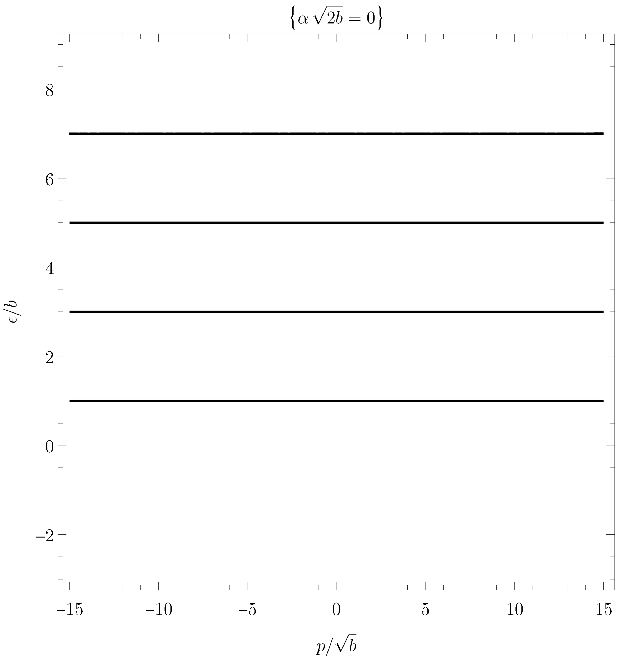
\includegraphics[width=0.45\textwidth]{grafy/dirac0.pdf}%
    \hspace{0.1\textwidth}%
    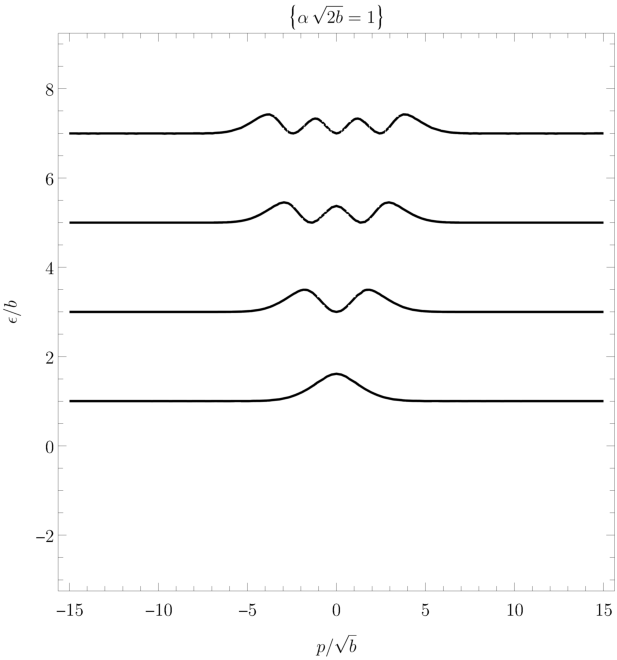
\includegraphics[width=0.45\textwidth]{grafy/dirac1.pdf}%
    \\[1em]%
    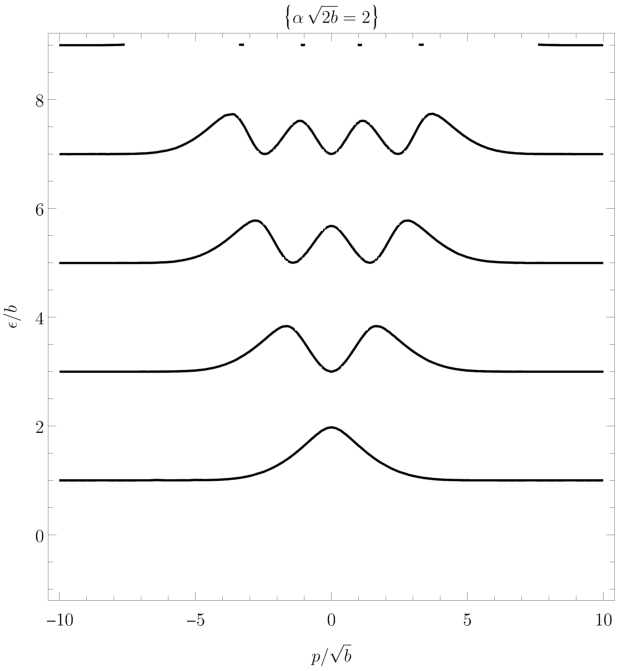
\includegraphics[width=0.45\textwidth]{grafy/dirac2.pdf}%
    \hspace{0.1\textwidth}%
    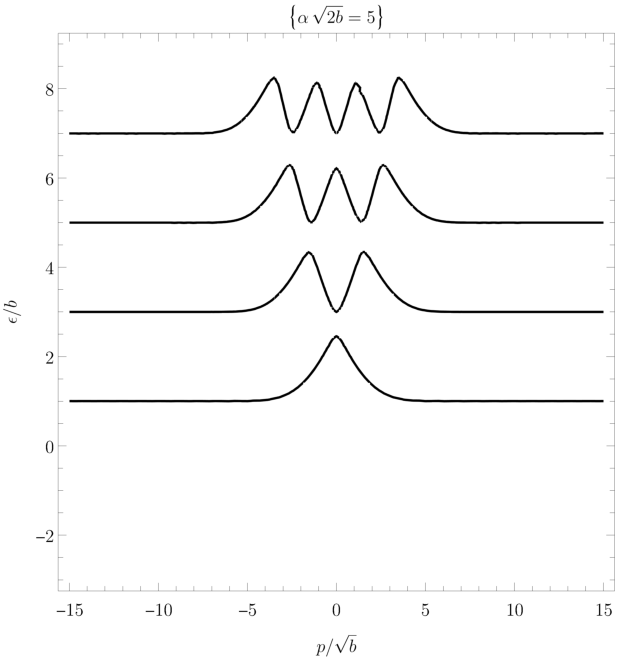
\includegraphics[width=0.45\textwidth]{grafy/dirac5.pdf}%
    \\[1em]%
    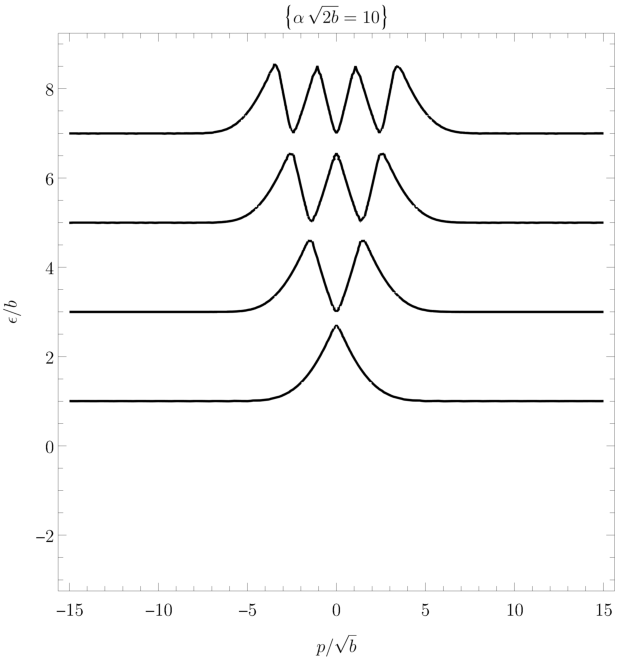
\includegraphics[width=0.45\textwidth]{grafy/dirac10.pdf}%
    \hspace{0.1\textwidth}%
    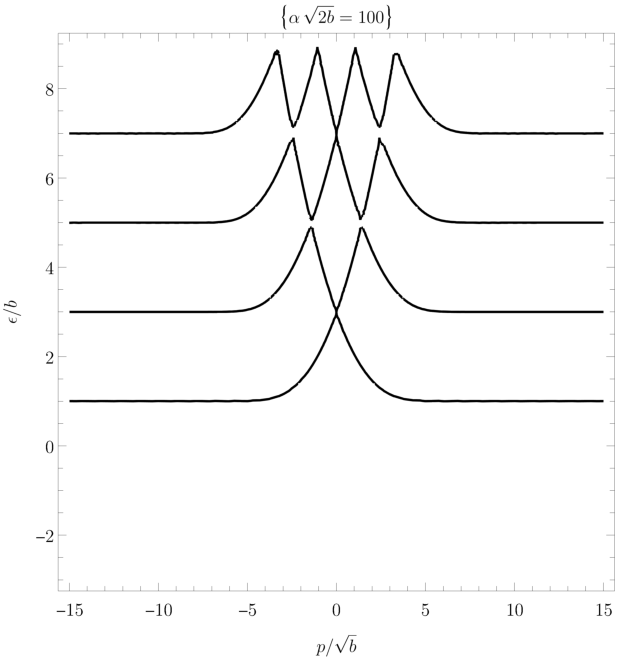
\includegraphics[width=0.45\textwidth]{grafy/dirac100.pdf}\par
    \caption{The first four energy levels $\epsilon$ as a function of the $y$-momentum $p$ for $\alpha\,\sqrt{2b} = 0, 1, 2, 5, 10$ and $100$ (starting with an unperturbed system, followed by an increasingly repulsive perturbation).}
    \label{plots-dirac-repulsive}
\end{figure}

\begin{figure}[p]
    \centering
    \noindent
    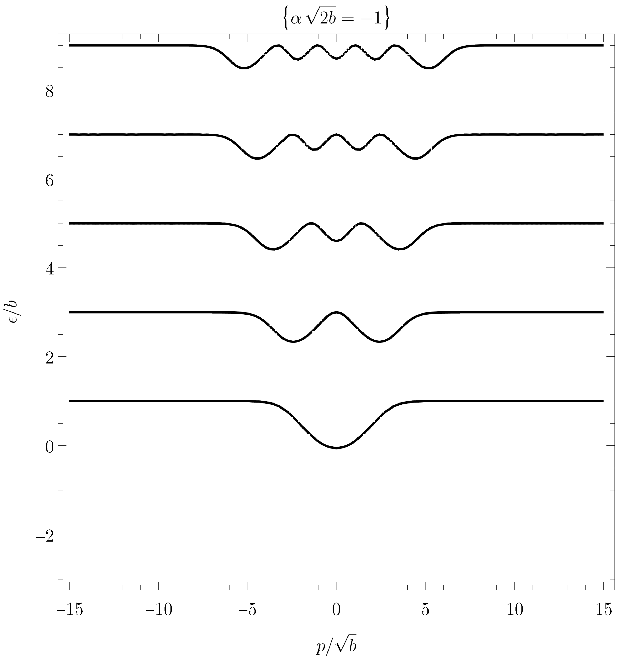
\includegraphics[width=0.45\textwidth]{grafy/dirac-1.pdf}%
    \hspace{0.1\textwidth}%
    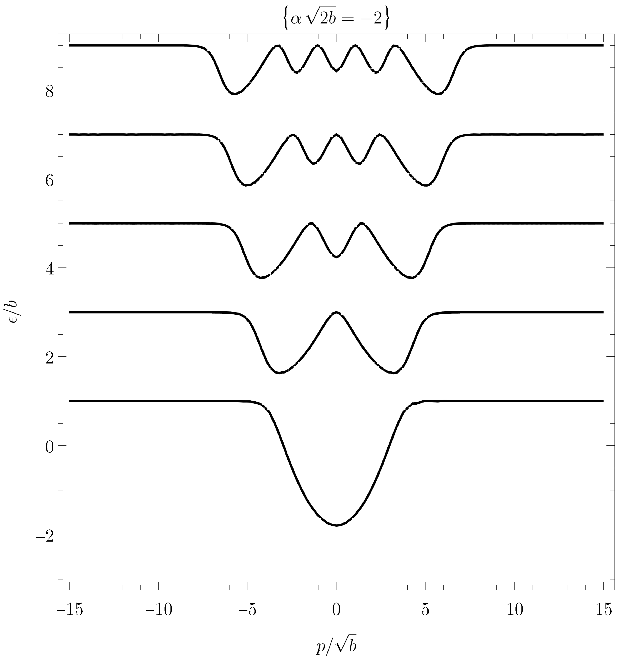
\includegraphics[width=0.45\textwidth]{grafy/dirac-2.pdf}%
    \\[2em]%
    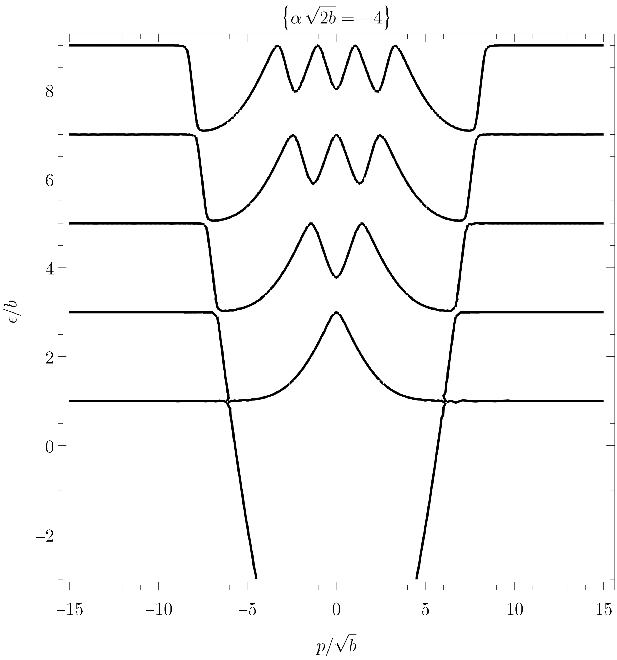
\includegraphics[width=0.45\textwidth]{grafy/dirac-4.pdf}%
    \hspace{0.1\textwidth}%
    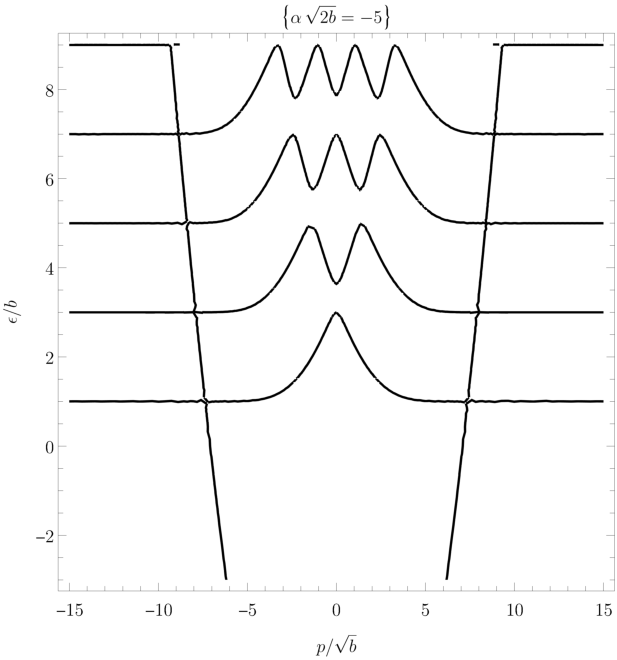
\includegraphics[width=0.45\textwidth]{grafy/dirac-5.pdf}\par
    \caption{The first five energy levels $\epsilon$ as a function of the $y$-momentum $p$ for $\alpha\,\sqrt{2b} = -1, -2, -4$ and $-5$ (system with an increasingly attractive perturbation).}
    \label{plots-dirac-attractive}
\end{figure}

\bigskip

For each fixed $\alpha$, the relation \eqref{eqn-dirac-epsilon-F-relation} defines a set of non-intersecting analytic functions $\big\{ \epsilon_0(p), \epsilon_1(p), ... \big\}$ defined on the entire $\R$. This can be demonstrated either from the properties of $F$ via the implicit mapping theorem (listed as 8.6 in \cite{KaupKaup1983}), or from the properties of $\Hf_\alpha(p)$ via Theorem \ref{thm-eigenval-holo}. We choose the latter approach:
\begin{equation*}
    \Hf_\alpha(p)
    = -\dd{^2}{x^2} + \big( b \, x + p \big)^2
    = \Hf_\alpha(0) + 2bp \, x + p^2
\end{equation*}
The fibre Hamiltonian is clearly holomorphic in $p$ and meets the assumptions of Theorem \ref{thm-eigenval-holo} for all $p \in \R$.

It is also true that the energy levels tend to the unperturbed Landau levels $\epsilon_k(p) \to (2k + 1)\, b$ as $p \to \pm \infty$. This follows from the fact that shifting $p$ by a constant amount is equivalent to changing $x_0$. Or more precisely, the fibre Hamiltonian $\Hf_{\alpha, \, x_0}(p)$ is unitarily equivalent to $\Hf_{\alpha, \, x_0 \, + \, p/b}(0)$. The bound states are concentrated around $x=0$ and decay exponentially away from it. Therefore, moving the point interaction further from $x=0$ will cause it to have a diminishing effect, completely vanishing at infinity.

We want to investigate, whether the functions $\epsilon_k(p)$ touch (or even cross) their respective Landau levels. From \eqref{eqn-dirac-epsilon-F-relation} we know that $\epsilon(p) = (2k + 1) \, b$ has a solution precisely if
\begin{equation*}
    F(a, w, k) = 0
    \qquad \text{ for some } w \in \R
    \: .
\end{equation*}
Using \eqref{eqn-parabolic-cylinder-hermite} and the fact that $H_k(-x) = (-1)^k \, H_k(x)$, we get:
\begin{align*}
    F(a, w, k)
    &=
    D_k(w) \, D_{k+1}(-w)
    \;+\; D_k(-w) \, D_{k+1}(w)
    \;+\; a \, D_k(w) \, D_k(-w)
    \\[10pt]
    &= 2^{-\frac{k}{2}-\frac{k+1}{2}} \;
    \e{-\frac{w^2}{4}-\frac{w^2}{4}} \;
    \Big(
        H_k\big(\tfrac{w}{\sqrt{2}}\big)
        H_{k+1}\big(\tfrac{-w}{\sqrt{2}}\big)
        +
        H_k\big(\tfrac{-w}{\sqrt{2}}\big)
        H_{k+1}\big(\tfrac{w}{\sqrt{2}}\big)
    \Big)
    \\
    &+ a \;
    2^{-\frac{k}{2}-\frac{k}{2}} \;
    \e{-\frac{w^2}{4}-\frac{w^2}{4}} \;
    H_k\big(\tfrac{w}{\sqrt{2}}\big)
    H_k\big(\tfrac{-w}{\sqrt{2}}\big)
    \\[-5pt]
    &= 2^{-k-\frac{1}{2}} \;
    \e{-\frac{w^2}{2}} \;
    (-1)^{k+1}
    \Big(
        \overbrace{
            H_k\big(\tfrac{w}{\sqrt{2}}\big)
            H_{k+1}\big(\tfrac{w}{\sqrt{2}}\big)
            -
            H_k\big(\tfrac{w}{\sqrt{2}}\big)
            H_{k+1}\big(\tfrac{w}{\sqrt{2}}\big)
        }^0
    \Big)
    \\
    &+ a \;
    2^{-k} \;
    \e{-\frac{w^2}{2}} \;
    (-1)^k \;
    H_k\big(\tfrac{w}{\sqrt{2}}\big)
    H_k\big(\tfrac{w}{\sqrt{2}}\big)
    \\[10pt]
    &= a \;
    (-1)^k \;
    2^{-k} \;
    \e{-( p \, + \, b x_0)^2 / b} \;
    \Big( H_k\big(\tfrac{p \, + \, b x_0}{\sqrt{b}}\big) \Big)^2
    \: .
\end{align*}
Unsurprisingly, for $a = \alpha \sqrt{2b} = 0$ the expression is zero. This reflects the fact that $\alpha = 0$ is the unperturbed system with constant energy levels $\epsilon_k(p) = (2k+1)b$. For $\alpha \neq 0$, there are several important observations we can make. First, if both $a$ and $k$ are constant, the sign of the expression doesn't change – it is either nonnegative or nonpositive – which means that the functions $\epsilon_k(p)$ never cross the Landau levels.\footnote{The sign of $F$ clearly flips between the energy levels, it is positive above/below each $\epsilon_k(p)$ and negative on the other side. Therefore, if $\epsilon_k(p)$ were to cross the Landau level, the sign of $F$ would have to change.} Second, for given $\alpha \neq 0$, either all energy functions are above their Landau level, or all are under it – this follows from the fact that the sign of $F$ alternates when incrementing $k$. Third, we can tell how many times each $\epsilon_k(p)$ touches the Landau level; such points must satisfy
\begin{equation*}
    F(a, w = \sqrt{2b} ( x_0 + \tfrac{p}{b} ), \, k) =
    a \;
    (-1)^k \;
    2^{-k} \;
    \e{-( p \, + \, b x_0)^2 / b} \;
    \Big( H_k\big(\tfrac{p \, + \, b x_0}{\sqrt{b}}\big) \Big)^2
    = 0
    \: .
\end{equation*}
And because the $k$-th Hermite polynomial $H_k$ has precisely $k$ roots, we know that the $k$-th Landau level touches an energy function in $k$ distinct points and these points do not depend on the value of $\alpha$.

Finally, we can make the following observation:
\begin{claim}
    If $\alpha \neq 0$, then each energy function $\epsilon_k(p)$ is not constant on any interval and its supremum is strictly less than the infimum of $\epsilon_{k+1}$.
\end{claim}
\begin{proof}
    We have shown that $\epsilon_k$ are analytic – an analytic function which is constant on an interval is constant everywhere. However, we know that $\epsilon_k(p) \neq b \, (2k+1)$ almost everywhere, yet $\epsilon_k(p) \to (2k+1)$, hence it is constant nowhere.

    The fact that the $k$-th Landau level touches an energy function $k$ times for any $\alpha \neq 0$, even infinitesimally small, implies that each $\epsilon_k$ touches \textit{its own} Landau level. There is no $\epsilon_k(p)$ that touches the $(k\pm 1)$-th Landau level – if there were one, it would have to touch the Landau level exactly at the same point as $\epsilon_{k\pm 1}(p)$, because the touching points do not depend on $\alpha$. However, this would violate the non-intersection of energy levels. Combined with the fact that all energy functions are above (or below) their Landau levels, this proves that there is a gap between the extrema of adjacent energy functions.
\end{proof}

\begin{claim}
    If $\alpha > 0$, then $\epsilon_k \geq b \, (2k+1)$, and if $\alpha < 0$, then $\epsilon_k \leq b \, (2k+1)$.
\end{claim}
\begin{proof}
    We have already shown that all energy functions are either above or below their Landau levels. Now, which is it? This question can be decided using the quadratic form of $\Hf_\alpha(p)$. Let $\alpha < \beta$, then:
    \begin{align*}
        (\varphi, \, \Hf_\alpha(p) \, \varphi)
        &= -\int_\R \overline{\varphi} \varphi''
        + \int_\R (b x + p)^2 \;\, \big|\varphi(x)\big|^2 \; \d{x}
        \\[5pt]
        &= \alpha \, \big|\varphi(x_0)\big|^2
        + \norm{\varphi'}_{L^2(\R)}^2
        + \norm{\varphi}_{L^2_{(bx+p)^2}(\R)}
        \\[5pt]
        &\leq \beta \, \big|\varphi(x_0)\big|^2
        + \norm{\varphi'}_{L^2(\R)}^2
        + \norm{\varphi}_{L^2_{(bx+p)^2}(\R)}
        =
        (\varphi, \, \Hf_\beta(p) \, \varphi)
        \: .
    \end{align*}
    The quadratic form of $\Hf_\alpha(p)$ is clearly nondecreasing in $\alpha$. Therefore, the energy functions will be under the Landau level for $\alpha$ negative and above it for $\alpha$ positive.
\end{proof}

Now, we have all we need to characterize the spectrum of $H_\alpha$ using Theorem~\ref{thm-direct-integral-spectrum}. If $\alpha \neq 0$, the pure point spectrum is clearly empty, because the functions $\epsilon_k(p)$ are not constant, hence the set $\{ p \; | \; \epsilon(p) = E \}$ has measure zero for every $E$. Furthermore, as $H_\alpha$ is a direct integral of an analytic operator-valued function $\Hf_\alpha(p)$ whose spectrum is discrete, the singular continuous spectrum of $H_\alpha$ is also empty, as proven by \cite{Filonov2006}. Thus, the spectrum of $H_\alpha$ will be entirely absolute continuous, consisting of disjoint bands spanning from the Landau levels up (for $\alpha>0$) or down (for $\alpha<0$).

\section{Summary}
The following theorem summarizes the information obtained about the spectrum of the Landau Hamiltonian with a Dirac delta perturbation:
\begin{thm}
    Let $\alpha, \, b$ and $H_\alpha$ be as in Definition~\ref{defn-hamiltonian-dirac}. If $\alpha>0$, then for each $k \in \N_0$ there exists $E_k \in (0, 2)$ such that
    \begin{equation*}
        \Sp(H_\alpha) = \SpAc(H_\alpha) =
        \bigcup_{k \in \N_0}
        \big[ b \, (2k+1), \; b \, (2k+1+E_k) \big]
        \: .
    \end{equation*}
    If $\alpha<0$, then there exists $E_0 \in (0, \infty)$ and for each $n \in \N$ there is $E_n \in (0, 2)$ such that
    \begin{equation*}
        \Sp(H_\alpha) = \SpAc(H_\alpha) =
        \bigcup_{k \in \N_0}
        \big[ b \, (2k+1-E_k), \; b \, (2k+1) \big]
        \: .
    \end{equation*}
\end{thm}
